\chapter{Prova de conceito}
\section{Ferramentas Pesquisadas}
\subsection{LegoLog}
O LegoLog baseia-se em dois componentes principais: um robô construído usando RIS (Robotics Invention System) e um controlador robótico Golog. A idéia básica por trás do RIS é que programas sejam construídos no computador e transferidos para o robô através de uma torre de infravermelho, que está ligada à porta serial do computador. A LEGO fornece um software base, conhecido como firmware, que implementa uma máquina virtual que pode ser baixada para o robô.  Esta máquina virtual permite que sejam escolhidos até cinco programas, cada um com até 32 variáveis, 8 tarefas e 9 sub-rotinas. Uma vez que o firmware está funcionando, é possível utilizar o próprio ambiente de programação no Windows, disponibilizado pela LEGO, para escrever programas para essa máquina virtual \cite{levesque2000legolog}. 

Porém, o LegoLog funciona apenas no antigo robô da LEGO, o RCX, que era quem utilizava essa torre de infravermelho para transmitir dados do computador para o robô. Como o objeto de estudo dessa proposta é o robô LEGO Mindstorms NXT, o LegoLog foi descartado como opção de ferramenta a ser utilizada por esse projeto.

\subsection{MLP}
A MLP é uma plataforma multiliguagens, criada em 2008, na Universidade de Madeira, por um projeto chamado DROIDE. Tem por principal objetivo criar uma biblioteca comum para a programação do kit LEGO Mindstorms NXT em diversas linguagens. Atualmente tem suporte para as seguintes linguagens de programação: C$++$, C\#, Visual Basic, Java e Prolog, e funciona apenas no sistema operacional Windows. 

Essa ferramenta consiste em um módulo base de comunicação, utilizado para todas as linguagens, e módulos separados, para cada linguagem individualmente. No módulo Prolog, é utilizada para programação a IDE SWIProlog, sendo necessário apenas, segundo a documentação\footnote{http://www.cee.uma.pt/droide2/plataforma/documentation/userguide.pdf} da plataforma, importar a biblioteca NXT.Prolog utilizando o comando use\_foreign\_library$/$1 disponível no próprio SWIProlog. 

Na documentação da MLP não contêm instruções de como utilizar os predicados na plataforma, nem tampouco como conectar a plataforma ao robô. Vários e-mails foram mandados para os criadores da plataforma, mas sem nenhuma resposta. Assim sendo, a MLP também foi descartada como opção de ferramenta a ser utilizada por esse projeto.

\subsection[PLNXT]{PLNXT}
Como descrito no capítulo de suporte tecnológico o PLNXT é uma plataforma baseada na \textit{Prolog API for Mindstorms NXT}, desenvolvida dentro do projeto \textit{HeKatE}\footnote{hekate.ia.agh.du.pl}, e visa proporcionar uma solução para a programação de alto nível no robô LEGO Mindstorms NXT. Alguns dos objetivos da plataforma são:
\begin{itemize}
\item Suportar todos os componentes do NXT padrão, como sensores e motores;
\item Ser uma solução multiplataforma, Windows e GNU/Linux;
\end{itemize}
A plataforma é composta por três camadas principais:
\begin{itemize}
\item Camada de comunicação (nxt\_actions): proporciona a comunicação de baixo nível com o robô;
\item Camada sensomotoric (nxt\_sensomoto): permite a troca de informações com sensores e motores;
\item Camada comportamental (nxt\_movement): fornece funções para controle do robô.
\end{itemize}
A comunicação com o robô pode ser feita via porta USB ou via Bluetooth. No site\footnote{http://ai.ia.agh.edu.pl/wiki/mindstorms:plnxt:start} do PLNXT é possível encontrar um tutorial passo-a-passo de como configurar o ambiente para utilizar a plataforma, além de códigos para testar a conexão, os motores e os sensores.

A configuração do ambiente para utilizar essa plataforma neste trabalho foi feita porém ao testar a conexão via bluetooth com o robô, utilizando o código disponibilizado no site, ocorre um problema, onde o robô identifica que está conectado ao computador mas a plataforma não identifica o robô. Apesar deste contra tempo, essa platafoma foi a escolhida para ser utilizada nesse trabalho.

\section{Descrição da prova de conceito}
\subsection{Problema da mochila}
O problema da mochila é um dos mais famosos problemas de otimização, onde existem vários objetos, que contêm um peso e um valor associado, e uma mochila com uma capacidade máxima que deve ser preenchida de forma que contenha o maior valor possível. Existem duas variações desse problema: a mochila binária e a mochila fracionária.

No caso da mochila binária é possível pegar somente todo o objeto ou não pegá-lo. Já a mochila fracionária é possível pegar parte de um objeto, mantendo a proporcionalidade do valor. Pode-se resolver esses problemas de várias formas, mas foi analisado por esse trabalho a resolução pelo algoritmo guloso e por programação dinâmica, segundo os dados a seguir.

\FloatBarrier
\begin{table}[h]
	\centering	
	\begin{tabular}{lccc}
		\toprule
		& \textbf{Item A} & \textbf{Item B} & \textbf{Item C} \\
		\midrule
		\textbf{valor} & 60 & 100 & 120 \\
		\midrule
		\textbf{peso} & 10 & 20 & 30 \\
		\midrule
		\textbf{valor/peso} & 6 7 5 & 4 \\
		\bottomrule
	\end{tabular}
	\caption{Problema da mochila}
	\label{knapsack}
\end{table}


\subsubsection{Resolução por algoritmo guloso}
Na resolução utilizando o algoritmo guloso, a melhor ordenação de entrada seria pelo valor/peso de forma decrescente. Dessa forma para o problema da mochila fracionária teríamos uma solução com um valor máximo alcançado de 240, de acordo com a Figura \ref{mochila}.

\FloatBarrier
\begin{figure}[!h]
\centering
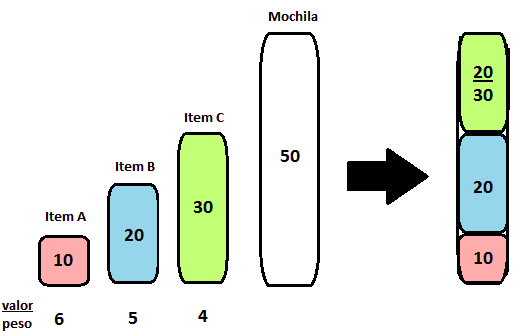
\includegraphics[keepaspectratio=true,scale=0.5]{figuras/mochila.png}
\caption{Problema da mochila fracionária - Algoritmo Guloso}
\label{mochila}
\end{figure}

E para a mochila binária o valor máximo alcançado seria de 160 como mostra a Figura \ref{mochilabinaria}.

\FloatBarrier
\begin{figure}[!h]
\centering
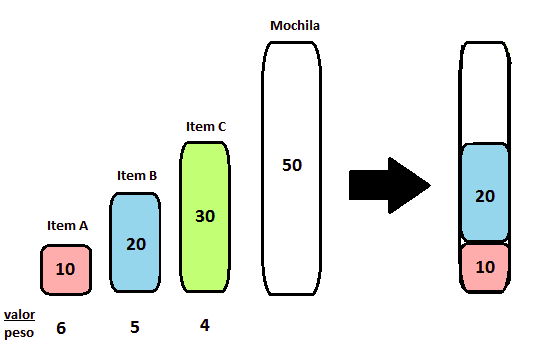
\includegraphics[keepaspectratio=true,scale=0.5]{figuras/mochilabinaria.png}
\caption{Problema da mochila binária - Algoritmo Guloso}
\label{mochilabinaria}
\end{figure}
\clearpage

Como é possível perceber, na resolução da mochila binária o algoritmo guloso não obtém sucesso, ja que a melhor solução teria o valor máximo igual 220, como demonstra a Figura \ref{mochilabinariacerta}.

\FloatBarrier
\begin{figure}[!h]
\centering
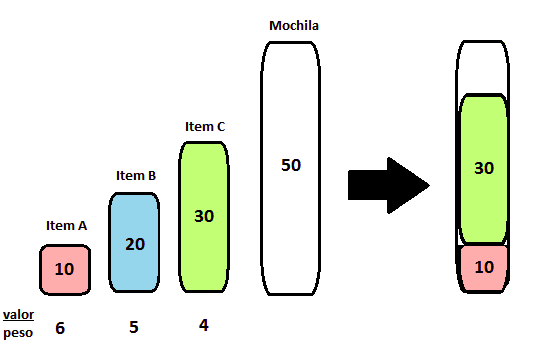
\includegraphics[keepaspectratio=true,scale=0.5]{figuras/mochilabinariacerta.png}
\caption{Problema da mochila binária - Resposta}
\label{mochilabinariacerta}
\end{figure}

\subsubsection{Resolução por programação dinâmica}
Na resolução da mochila binária por programação dinâmica, é criada uma matriz onde as linhas são os itens e as colunas é a capacidade da mochila ordenada de forma crescente. No caso do exemplo anteriormente citado, seria criada uma matriz igual a mostrada na Figura \ref{matriz}.

\FloatBarrier
\begin{figure}[!h]
\centering
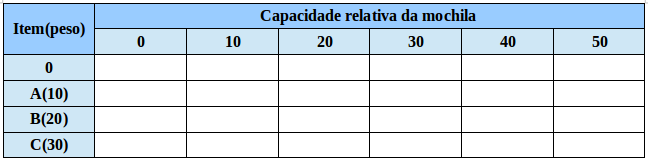
\includegraphics[keepaspectratio=true,scale=0.5]{figuras/matriz.png}
\caption{Problema da mochila binária - Programação Dinâmica}
\label{matriz}
\end{figure}

A análise se inicia na primeira célula (linha 1, coluna 1), e a cada passo vai analisando a próxima célula da linha, quando chega ao final, volta a primeira coluna e desce para a segunda linha, caracterizando uma análise \textit{top-down}. 

A cada iteração é analisado primeiramente o peso do item em relação a capacidade relativa da mochila (referente a coluna que se está analisando), podendo resultar em três cenários: 
\begin{enumerate}
\item \textbf{Peso analisado é igual a capacidade relativa:} nesse cenário o algoritmo se pergunta: O que é melhor? Tomar o valor da célula anterior, tomar o valor da célula acima ou tomar o valor do item analisado? Após a decisão ele grava o valor na matriz.
\item \textbf{Peso analisado é inferior a capacidade relativa:} nesse cenário o algoritmo se pergunta: É melhor tomar o valor da célula acima ou é melhor tomar o valor do item analisado somado a célula da linha acima que complemente o peso analisado, de forma que a capacidade relativa seja alcançada? Após tomada a decisão, ele grava o valor na matriz. 
\item \textbf{Peso analisado é superior a capacidade relativa:} nesse cenário não é possível tomar o valor do item analisado, logo, o algoritmo se pergunta: é melhor tomar o valor da célula ao lado ou da célula acima? 
\end{enumerate}

Dada uma matriz (NxM) a última célula da mesma (linha N, coluna M) contém a resposta para o problema analisado. 

Tomando como exemplo a Tabela \ref{knapsack}, a solução por programação dinâmica cria uma matriz como a da Figura \ref{matriz} e preenche a primeira linha e a primeira coluna com zeros, como mostra a Figura \ref{matrizZero} pois se a capacidade da mochila é zero (primeira coluna) não tem como pegar nenhum item, e se não tem nenhum item para analisar (primeira linha) não tem como tomar nenhum valor. Mesmo na prática não existindo uma mochila sem capacidade ou nenhum item para ser analisado, essas hipóteses são acrescentadas para que na hora da execução do algoritmo não ocorra nenhum erro, já que ele está sempre analisando o valor de outras células para a tomada de decisão.

\FloatBarrier
\begin{figure}[!h]
\centering
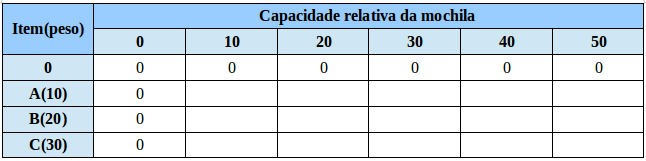
\includegraphics[keepaspectratio=true,scale=0.5]{figuras/matrizZero.png}
\caption{Problema da mochila binária - PD - Passo Inicial}
\label{matrizZero}
\end{figure}

O segundo passo é analisar a capacidade da mochila sendo 10, e havendo apenas o item A, com peso 10. Logo, tem-se o cenário do peso analisado igual à capacidade relativa, e obviamente, o melhor, nesse caso, é tomar o valor do item analisado, ou seja, escrever 60 na célula, como mostra a Figura \ref{matriz60}.

\FloatBarrier
\begin{figure}[!h]
\centering
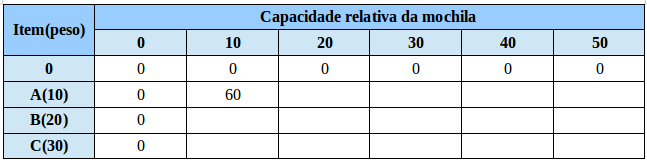
\includegraphics[keepaspectratio=true,scale=0.5]{figuras/matriz60.png}
\caption{Problema da mochila binária - PD - Item A, Capacidade 10}
\label{matriz60}
\end{figure}

Em seguida é analisada a capacidade da mochila como sendo 20. Nesse casso, existe apenas o item A, de peso 10, para ser colocado na mochila. Imediatamente é sabido, por nós humanos, que o valor desse item será escrito na célula, porém a progração dinâmica não tem esse conhecimento, e avalia o cenário de peso analisado inferior à capacidade relativa da mochila. Nesse cenário, é possível tomar o valor da célula acima, que é zero, ou o valor do item de peso 10 somado ao seu complemento, contido na linha acima, que o faz alcançar a capacidade da mochila. A coluna que complementa o peso do item é a de valor 10, pois assim é alcançado o valor 20 da capacidade relativa analisada. As Figuras \ref{matriz10_20} e \ref{matriz10_20_resp} demonstram essa decisão.

\FloatBarrier
\begin{figure}[!h]
\centering
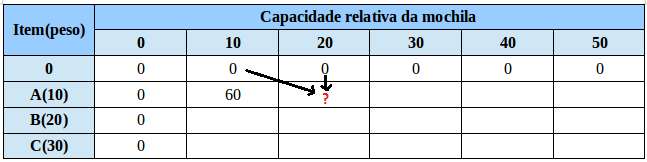
\includegraphics[keepaspectratio=true,scale=0.6]{figuras/matriz10_20.png}
\caption{Problema da mochila binária - PD - Item A, Capacidade 20 - Análise }
\label{matriz10_20}
\end{figure}

\FloatBarrier
\begin{figure}[!h]
\centering
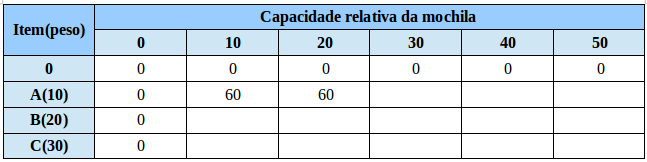
\includegraphics[keepaspectratio=true,scale=0.6]{figuras/matriz10_20_resp.png}
\caption{Problema da mochila binária - PD - Item A, Capacidade 20 - Resultado}
\label{matriz10_20_resp}
\end{figure}

Essa análise é feita para toda a linha, como mostram as Figuras \ref{matriz10_30}, \ref{matriz10_30_resp}, \ref{matriz10_40}, \ref{matriz10_40_resp}, \ref{matriz10_50} e \ref{matriz10_50_resp}, onde em todos os passos foi decidido, pela programação dinâmica, a soma do valor do item A, que é 60, e o seu complemento, que em todos os casos tem valor zero.

\FloatBarrier
\begin{figure}[!h]
\centering
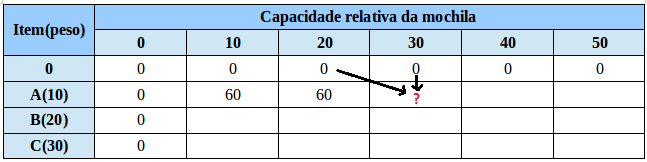
\includegraphics[keepaspectratio=true,scale=0.6]{figuras/matriz10_30.png}
\caption{Problema da mochila binária - PD - Item A, Capacidade 30 - Análise}
\label{matriz10_30}
\end{figure}

\FloatBarrier
\begin{figure}[!h]
\centering
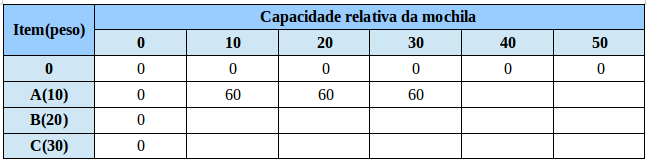
\includegraphics[keepaspectratio=true,scale=0.6]{figuras/matriz10_30_resp.png}
\caption{Problema da mochila binária - PD - Item A, Capacidade 30 - Resultado}
\label{matriz10_30_resp}
\end{figure} 

\FloatBarrier
\begin{figure}[!h]
\centering
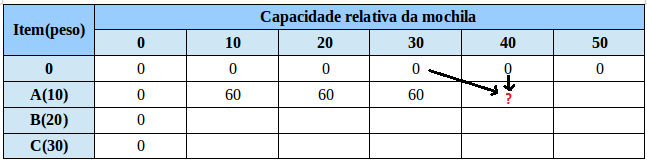
\includegraphics[keepaspectratio=true,scale=0.6]{figuras/matriz10_40.png}
\caption{Problema da mochila binária - PD - Item A, Capacidade 40 - Análise}
\label{matriz10_40}
\end{figure}

\FloatBarrier
\begin{figure}[!h]
\centering
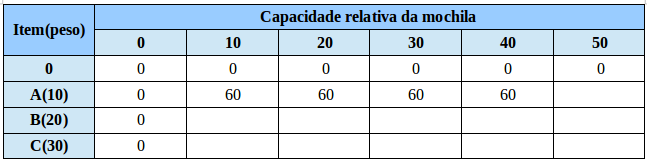
\includegraphics[keepaspectratio=true,scale=0.6]{figuras/matriz10_40_resp.png}
\caption{Problema da mochila binária - PD - Item A, Capacidade 40 - Resultado}
\label{matriz10_40_resp}
\end{figure}

\FloatBarrier
\begin{figure}[!h]
\centering
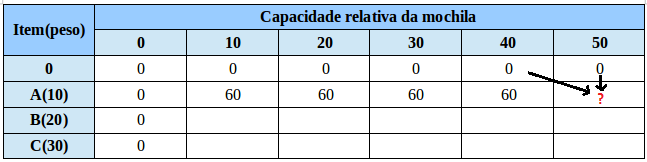
\includegraphics[keepaspectratio=true,scale=0.6]{figuras/matriz10_50.png}
\caption{Problema da mochila binária - PD - Item A, Capacidade 50 - Análise}
\label{matriz10_50}
\end{figure}

\FloatBarrier
\begin{figure}[!h]
\centering
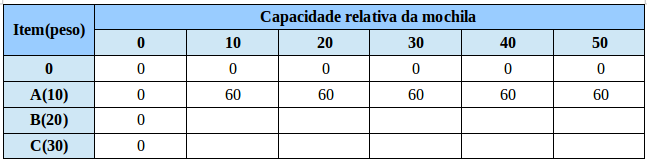
\includegraphics[keepaspectratio=true,scale=0.6]{figuras/matriz10_50_resp.png}
\caption{Problema da mochila binária - PD - Item A, Capacidade 50 - Resultado}
\label{matriz10_50_resp}
\end{figure}
 
A análise do item B, de peso 20, quando a capacidade da mochila é 10, é o cenário de peso analisado superior a capacidade relativa. Nesse caso, é possível continuar com o valor contindo na mochila na capacidade relativa anterior (célula anterior), ou pode-se tomar o valor do item anterior quando a capacidade relativa da mochila é a mesma (célula acima). Dessa forma, a programação dinâmica decide pela célula acima e escreve seu valor na célula analisada. As Figuras \ref{matriz20_10} e \ref{mochila20_10_resp} demonstra essa decisão.

\FloatBarrier
\begin{figure}[!h]
\centering
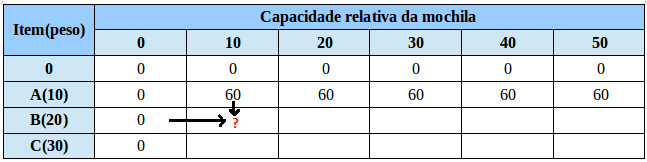
\includegraphics[keepaspectratio=true,scale=0.5]{figuras/matriz20_10.png}
\caption{Problema da mochila binária - PD - Item B, Capacidade 10 - Análise}
\label{matriz20_10}
\end{figure}

\FloatBarrier
\begin{figure}[!h]
\centering
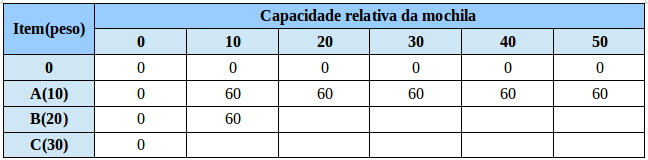
\includegraphics[keepaspectratio=true,scale=0.5]{figuras/mochila20_10_resp.png}
\caption{Problema da mochila binária - PD - Item B, Capacidade 10 - Resultado}
\label{mochila20_10_resp}
\end{figure}

As demais decisões são efetuadas seguindo um dos passo-a-passo anteriormente citados, dependendo do cenário que se está analisando. As Figuras \ref{mochila20_20}, \ref{mochila20_20_resp}, \ref{mochila20_30}, \ref{mochila20_30_resp}, \ref{mochila20_40}, \ref{mochila20_40_resp}, \ref{mochila20_50}, \ref{mochila20_50_resp}, \ref{mochila30_10}, \ref{mochila30_10_resp}, \ref{mochila30_20}, \ref{mochila30_20_resp}, \ref{mochila30_30}, \ref{mochila30_30_resp}, \ref{mochila30_40}, \ref{mochila30_40_resp}, \ref{mochila30_50} e \ref{mochila30_50_resp} demonstram tais decisões.
\FloatBarrier
\begin{figure}[!h]
\centering
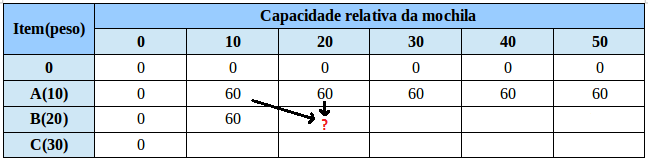
\includegraphics[keepaspectratio=true,scale=0.6]{figuras/mochila20_20.png}
\caption{Problema da mochila binária - PD - Item B, Capacidade 20 - Análise}
\label{mochila20_20}
\end{figure}

\FloatBarrier
\begin{figure}[!h]
\centering
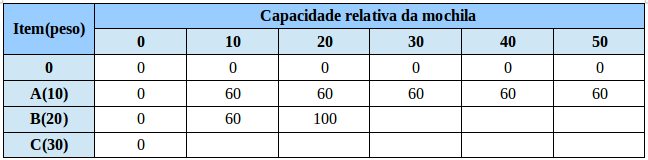
\includegraphics[keepaspectratio=true,scale=0.6]{figuras/mochila20_20_resp.png}
\caption{Problema da mochila binária - PD - Item B, Capacidade 20 - Resultado}
\label{mochila20_20_resp}
\end{figure}

\FloatBarrier
\begin{figure}[!h]
\centering
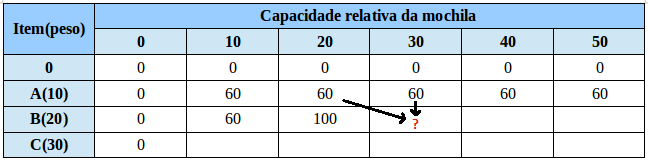
\includegraphics[keepaspectratio=true,scale=0.6]{figuras/mochila20_30.png}
\caption{Problema da mochila binária - PD - Item B, Capacidade 30 - Análise}
\label{mochila20_30}
\end{figure}

\FloatBarrier
\begin{figure}[!h]
\centering
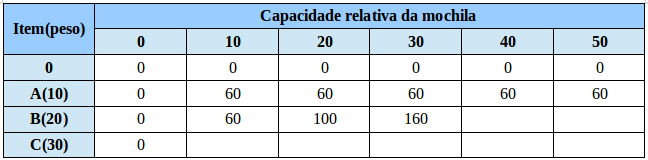
\includegraphics[keepaspectratio=true,scale=0.6]{figuras/mochila20_30_resp.png}
\caption{Problema da mochila binária - PD - Item B, Capacidade 30 - Resultado}
\label{mochila20_30_resp}
\end{figure}

\FloatBarrier
\begin{figure}[!h]
\centering
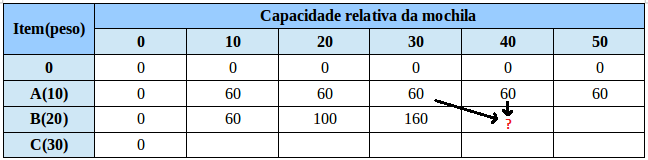
\includegraphics[keepaspectratio=true,scale=0.6]{figuras/mochila20_40.png}
\caption{Problema da mochila binária - PD - Item B, Capacidade 40 - Análise}
\label{mochila20_40}
\end{figure}

\FloatBarrier
\begin{figure}[!h]
\centering
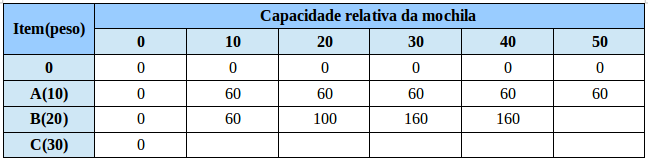
\includegraphics[keepaspectratio=true,scale=0.6]{figuras/mochila20_40_resp.png}
\caption{Problema da mochila binária - PD - Item B, Capacidade 40 - Resultado}
\label{mochila20_40_resp}
\end{figure}

\FloatBarrier
\begin{figure}[!h]
\centering
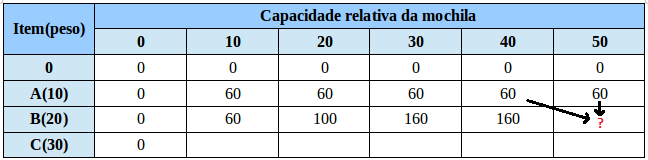
\includegraphics[keepaspectratio=true,scale=0.6]{figuras/mochila20_50.png}
\caption{Problema da mochila binária - PD - Item B, Capacidade 50 - Análise}
\label{mochila20_50}
\end{figure}

\FloatBarrier
\begin{figure}[!h]
\centering
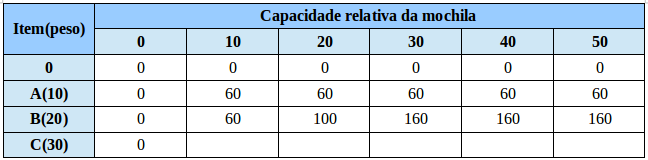
\includegraphics[keepaspectratio=true,scale=0.6]{figuras/mochila20_50_resp.png}
\caption{Problema da mochila binária - PD - Item B, Capacidade 50 - Resultado}
\label{mochila20_50_resp}
\end{figure}

\FloatBarrier
\begin{figure}[!h]
\centering
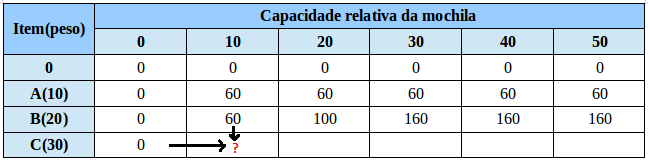
\includegraphics[keepaspectratio=true,scale=0.6]{figuras/mochila30_10.png}
\caption{Problema da mochila binária - PD - Item C, Capacidade 10 - Análise}
\label{mochila30_10}
\end{figure}

\FloatBarrier
\begin{figure}[!h]
\centering
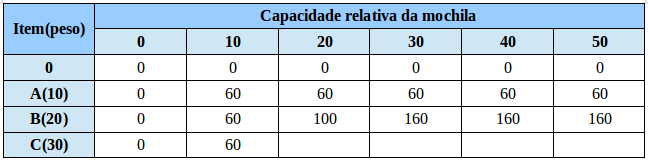
\includegraphics[keepaspectratio=true,scale=0.6]{figuras/mochila30_10_resp.png}
\caption{Problema da mochila binária - PD - Item C, Capacidade 10 - Resultado}
\label{mochila30_10_resp}
\end{figure}

\FloatBarrier
\begin{figure}[!h]
\centering
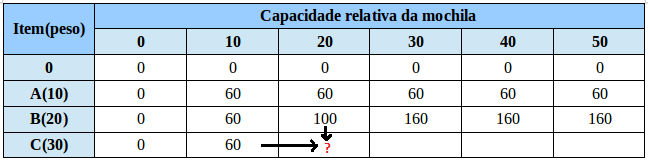
\includegraphics[keepaspectratio=true,scale=0.6]{figuras/mochila30_20.png}
\caption{Problema da mochila binária - PD - Item C, Capacidade 20 - Análise}
\label{mochila30_20}
\end{figure}

\FloatBarrier
\begin{figure}[!h]
\centering
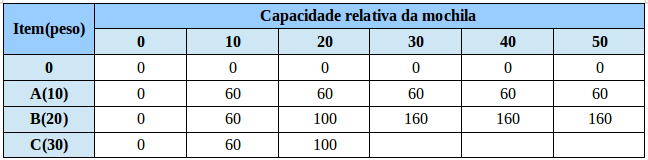
\includegraphics[keepaspectratio=true,scale=0.6]{figuras/mochila30_20_resp.png}
\caption{Problema da mochila binária - PD - Item C, Capacidade 20 - Resultado}
\label{mochila30_20_resp}
\end{figure}

As Figuras \ref{mochila30_30} e \ref{mochila30_30_resp} mostram a decisão da programação dinâmica quanto um cenário de peso analisado é igual a capacidade relativa da mochila, onde a melhor opção foi não foi tomar o valor do item, que seria 120, mas tomar o valor da do item anterior na mesma capacidade relativa (célula acima), que é 160.
\FloatBarrier
\begin{figure}[!h]
\centering
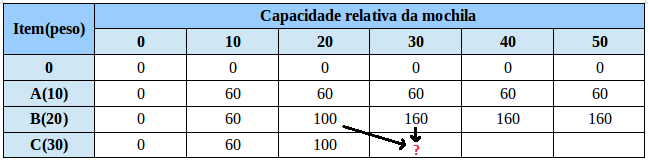
\includegraphics[keepaspectratio=true,scale=0.6]{figuras/mochila30_30.png}
\caption{Problema da mochila binária - PD - Item C, Capacidade 30 - Análise}
\label{mochila30_30}
\end{figure}

\FloatBarrier
\begin{figure}[!h]
\centering
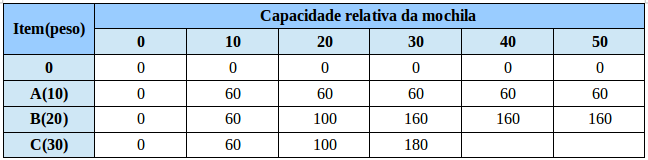
\includegraphics[keepaspectratio=true,scale=0.6]{figuras/mochila30_30_resp.png}
\caption{Problema da mochila binária - PD - Item C, Capacidade 30 - Resultado}
\label{mochila30_30_resp}
\end{figure}

\FloatBarrier
\begin{figure}[!h]
\centering
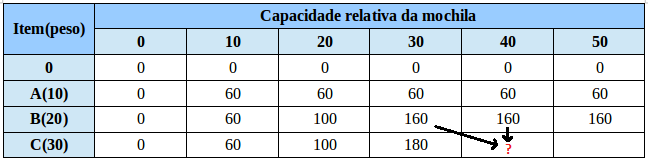
\includegraphics[keepaspectratio=true,scale=0.6]{figuras/mochila30_40.png}
\caption{Problema da mochila binária - PD - Item C, Capacidade 40 - Análise}
\label{mochila30_40}
\end{figure}

\FloatBarrier
\begin{figure}[!h]
\centering
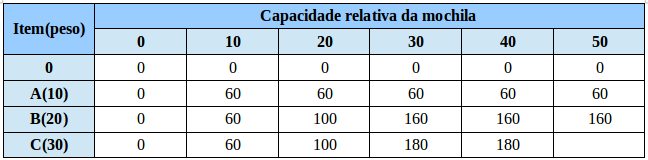
\includegraphics[keepaspectratio=true,scale=0.6]{figuras/mochila30_40_resp.png}
\caption{Problema da mochila binária - PD - Item C, Capacidade 40 - Resultado}
\label{mochila30_40_resp}
\end{figure}

\FloatBarrier
\begin{figure}[!h]
\centering
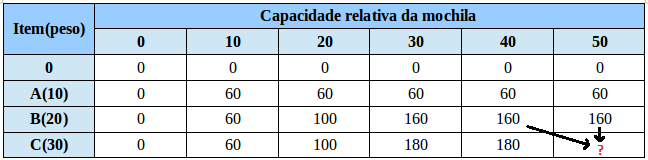
\includegraphics[keepaspectratio=true,scale=0.6]{figuras/mochila30_50.png}
\caption{Problema da mochila binária - PD - Item C, Capacidade 50 - Análise}
\label{mochila30_50}
\end{figure}

\FloatBarrier
\begin{figure}[!h]
\centering
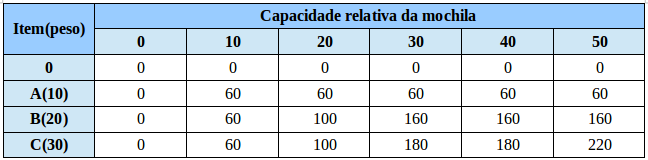
\includegraphics[keepaspectratio=true,scale=0.5]{figuras/mochilaResultado.png}
\caption{Problema da mochila binária - PD - Item C, Capacidade 50 - Resultado}
\label{mochila30_50_resp}
\end{figure}

O valor da última célula é a resposta para o problema. Como pode-se ver na Figura \ref{mochila30_50_resp}, o valor encontrado pela programação dinâmica foi 220, demonstrando que para o problema da mochila binária ele é eficaz.
 
\subsection{Adaptação do problema da mochila para o contexto do trabalho}
Para o completo entendimento do trabalho proposto algumas definições sobre termos amplamente utilizados no kit LEGO Mindstorms NXT se fazem necessárias e são feitas a seguir.
\begin{itemize}
\item \textbf{Missão:} uma missão é composta por uma tarefa que deve ser executada pelo robô em um determinado tempo, valendo uma pontuação, e por um trajeto que deve ser efetuado pelo robô para executar a missão;
\item \textbf{Pontuação da missão:} cada missão tem uma pontuação previamente estabelecida. Essa pontuação é alcançada se a missão for concluída comm sucesso;
\item \textbf{Pontuação total:} é o somatório das pontuações de todas as missões concluídas com sucesso;
\item \textbf{Mapa:} um mapa é onde o robô deve executar as missões. Cada mapa contém diferentes missões associados a ele;
\item \textbf{Tempo total:} é uma quantidade de tempo, previamente estabelecida, geralmente de dois a três minutos, utilizada para executar o máximo de missões possíveis almejando a maior pontuação total;
\item \textbf{Tempo restante:} é a quantidade de tempo que falta para chegar ao fim do tempo total;
\item \textbf{Tempo da tarefa:}  é a quantidade de tempo necessária para que o robô execute uma tarefa;
\item \textbf{Tempo do trajeto:} é a quantidade de tempo que o robô utiliza para chegar em um local com coordenadas (X, Y) partindo de um local com coordenadas (X0, Y0);
\item \textbf{Tempo da missão:} é a quantidade de tempo utilizada para concluir a missão com sucesso.
\item \textbf{Base:} Local no mapa de onde o robô deve partir para executar a primeira missão. 
\end{itemize}

O objetivo do trabalho é alcançar a maior pontuação dentro de um determinado espaço de tempo. Supondo que existam 3 missões para o robô executar, missão da árvore, missão dos pets e missão do avião, descritas a seguir, quais missões devem ser executadas, dentro de um tempo restante de 50 segundos, para se alcançar a maior pontuação?

\begin{itemize}
\item \textbf{Missão árvore:} Essa missão consiste de uma tarefa em que o robô tem que derrubar o galho de uma árvore, sem deixar que ele encoste nos fios de alta tensão. Tempo de execução da tarefa: 5 segundos; Tempo da trajetória: 5 segundos; Tempo da missão: Tempo da trajetória + tempo da tarefa = 10 segundos;
\item \textbf{Missão pets:} Essa missão consiste na tarefa de resgatar os pets e levá-los a base. Tempo de execução da tarefa: 10 segundos; Tempo da trajetória: 10 segundos; Tempo da missão: 20 segundos;
\item \textbf{Missão avião}: Essa missão consiste na tarefa de derrubar o avião na pista de pouso; Tempo de execução da tarefa: 10 segundos; Tempo da trajetória: 20 segundos; Tempo de execução da missão: 20 segundos;
\end{itemize}

Da mesma forma que no problema da mochila binária não é possível pegar uma fração de um objeto, no contexto desse trabalho não é possível executar uma fração de uma missão, tornando o problema binário para ganhar a pontuação da missão. Desta forma é criada uma matriz onde o eixo X é o tempo restante e o eixo Y é o tempo de execução de cada missão, como mostra a Figura \ref{matrizProlego}.

\FloatBarrier
\begin{figure}[!h]
\centering
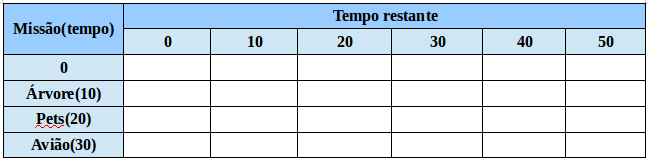
\includegraphics[keepaspectratio=true,scale=0.6]{figuras/matrizProlego.png}
\caption{Prolego - Programação Dinâmica}
\label{matrizProlego}
\end{figure}


Resolvendo essa matriz com programação dinâmica é alcançado o valor de 220, como mostra a Figura \ref{matrizProlegoResult}, ou seja, as missões que devem ser executadas são: missão pets e missão avião.  

\FloatBarrier
\begin{figure}[!h]
\centering
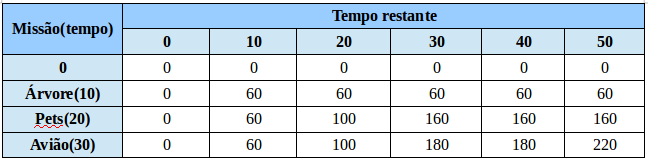
\includegraphics[keepaspectratio=true,scale=0.6]{figuras/matrizProlegoResult.png}
\caption{Prolego - Programação Dinâmica - Resultado}
\label{matrizProlegoResult}
\end{figure}


